\chapter{Error Correction Techniques and Digital Audio Recording}
\makeheading{2020-04-01}
\section{Reed-Solomon Codes}
Invented by Irving Reed and Gustave Solomon in 1960.

\begin{figure}[!htbp]
    \centering
    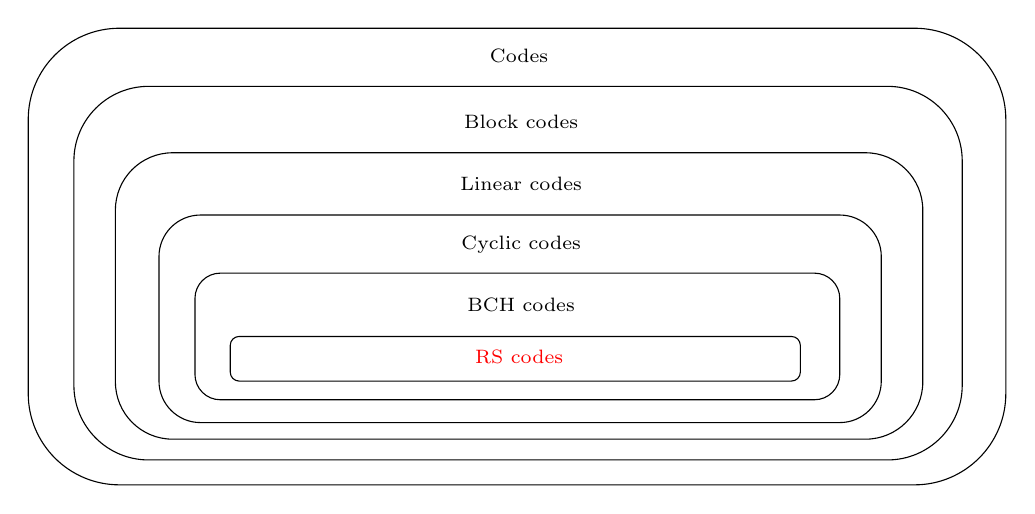
\begin{tikzpicture}[x=0.75pt,y=0.75pt,yscale=-1,xscale=1]
        %uncomment if require: \path (0,252); %set diagram left start at 0, and has height of 252

        %Rounded Rect [id:dp9312296811993294] 
        \draw   (79,55) .. controls (79,30.7) and (98.7,11) .. (123,11) -- (506,11) .. controls (530.3,11) and (550,30.7) .. (550,55) -- (550,187) .. controls (550,211.3) and (530.3,231) .. (506,231) -- (123,231) .. controls (98.7,231) and (79,211.3) .. (79,187) -- cycle ;
        %Rounded Rect [id:dp5374802904094965] 
        \draw   (101,75) .. controls (101,55.12) and (117.12,39) .. (137,39) -- (493,39) .. controls (512.88,39) and (529,55.12) .. (529,75) -- (529,183) .. controls (529,202.88) and (512.88,219) .. (493,219) -- (137,219) .. controls (117.12,219) and (101,202.88) .. (101,183) -- cycle ;
        %Rounded Rect [id:dp5846257319304448] 
        \draw   (121,98.6) .. controls (121,83.36) and (133.36,71) .. (148.6,71) -- (482.4,71) .. controls (497.64,71) and (510,83.36) .. (510,98.6) -- (510,181.4) .. controls (510,196.64) and (497.64,209) .. (482.4,209) -- (148.6,209) .. controls (133.36,209) and (121,196.64) .. (121,181.4) -- cycle ;
        %Rounded Rect [id:dp050418068340879474] 
        \draw   (142,121) .. controls (142,109.95) and (150.95,101) .. (162,101) -- (470,101) .. controls (481.05,101) and (490,109.95) .. (490,121) -- (490,181) .. controls (490,192.05) and (481.05,201) .. (470,201) -- (162,201) .. controls (150.95,201) and (142,192.05) .. (142,181) -- cycle ;
        %Rounded Rect [id:dp04503017510855856] 
        \draw   (159.33,141.2) .. controls (159.33,134.46) and (164.79,129) .. (171.53,129) -- (457.8,129) .. controls (464.54,129) and (470,134.46) .. (470,141.2) -- (470,177.8) .. controls (470,184.54) and (464.54,190) .. (457.8,190) -- (171.53,190) .. controls (164.79,190) and (159.33,184.54) .. (159.33,177.8) -- cycle ;
        %Rounded Rect [id:dp5932736850882949] 
        \draw   (176.33,163.8) .. controls (176.33,161.43) and (178.25,159.5) .. (180.63,159.5) -- (446.7,159.5) .. controls (449.07,159.5) and (451,161.43) .. (451,163.8) -- (451,176.7) .. controls (451,179.07) and (449.07,181) .. (446.7,181) -- (180.63,181) .. controls (178.25,181) and (176.33,179.07) .. (176.33,176.7) -- cycle ;

        % Text Node
        \draw (315.5,24.5) node  [font=\scriptsize] [align=left] {Codes};
        % Text Node
        \draw (316.5,56.1) node  [font=\scriptsize] [align=left] {Block codes};
        % Text Node
        \draw (316.5,86.1) node  [font=\scriptsize] [align=left] {Linear codes};
        % Text Node
        \draw (316.5,115.1) node  [font=\scriptsize] [align=left] {Cyclic codes};
        % Text Node
        \draw (316.5,144.1) node  [font=\scriptsize] [align=left] {BCH codes};
        % Text Node
        \draw (315.5,169.5) node  [font=\scriptsize,color={rgb, 255:red, 255; green, 0; blue, 0 }  ,opacity=1 ] [align=left] {RS codes};
    \end{tikzpicture}
\end{figure}

\begin{Definition}{Reed-solomon code}{rs_code}
    A \textbf{Reed-Solomon (RS) code} is a BCH code
    of length $ n $ over $ GF(q) $ where $ n\mid (q-1) $.
    \begin{Remark}{}{}
        Since $ q^1 \equiv 1\mod n $, we have $ m=1 $.
    \end{Remark}
\end{Definition}

\begin{Example}{}{}
    Let $ q=2^4 $ and $ GF(2^4)=\mathbb{Z}_2/(\alpha^4+\alpha+1) $.
    Recall that $ \alpha $ is a generator of $ GF(2^4)^\star $.

    Let $ \beta=\alpha^3 $, then $ \ord(\beta)=5 $, (so $ q=16 $, $ n=5 $).

    Let
    \[ g(x)=\lcm \set[\big]{m_{\beta}(x),m_{\beta^2}(x),m_{\beta^3}(x)}
        =(x-\beta)(x-\beta^2)(x-\beta^3)
        =x^3+\alpha^{11}x^2+\alpha^2x+\alpha^3 \]
    Then, $ g(x) $ generates a $ (5,2) $-RS code $ C $ over $ GF(2^4) $
    with $ \delta=4 $. In fact, $ d(C)=4 $ since $ g(x) $
    is a codeword of weight $ 4 $.

    A generator matrix for $ C $ is
    \[ G=
        \begin{bmatrix}
            \alpha^3 & \alpha^2 & \alpha^{11} & 1           & 0 \\
            0        & \alpha^3 & \alpha^2    & \alpha^{11} & 1
        \end{bmatrix}_{2\times 5} \]
    Consider the code $ C^{\prime} $ obtained from $ C $
    by replacing each symbol in codewords of $ C $ by their binary vector representation.
    For example,
    \[ \text{e.g., }\quad(\alpha^3,\alpha^2,\alpha^{11},1,0)\longleftrightarrow (0001\; 0010\; 0111\; 1000\; 0000) \]
    It is not difficult to see that $ C^{\prime} $ is closed under vector addition and scalar
    multiplication over $ GF(2) $. Thus, $ C^{\prime} $ is a $ (20,8) $-binary code.
\end{Example}

\begin{Definition}{RS code $ \symbf{C} $ of length $ \symbf{n} $ over $ \symbf{GF(q)} $
        with designed distance $ \symbf{\delta} $}{}
    Suppose $ n\mid (q-1) $, and let $ \beta\in GF(q) $ be an element of order $ n $.
    Then, $ m_{\beta^i}(x)=x-\beta^i $ for all $ i $.

    \vspace{1mm}

    An
    \textbf{RS code $ \symbf{C} $ of length $ \symbf{n} $ over $ \symbf{GF(q)} $
        with designed distance $ \symbf{\delta} $} is a cyclic code over $ GF(q) $
    with generator polynomial
    \[ g(x)=(x-\beta^{a})(x-\beta^{a+1})(x-\beta^{a+2})\cdots
        (x-\beta^{a+\delta-2})\quad\text{for some $ a $.} \]
    Since $ \deg(g)=\delta-1 $, we have $ w(g)\leqslant \delta $,
    so $ d(C)\leqslant \delta $.
    By the BCH bound, $ d(C)\geqslant \delta $, hence $ d(C)=\delta $.
\end{Definition}
Since $ \dim(C)=k=n-\deg(g)=n-\delta+1 $, we have $ k=n-d+1 $,
so $ d=n-k+1 $. Recall that $ d\leqslant n-k+1 $ for any $ (n,k,d) $-code.
Thus, \emph{RS codes are optimal} in the sense that, for any fixed $ n,k,q $,
they achieve maximum distance among all $ (n,k,d) $-codes over $ GF(q) $.

\subsection*{RS Codes Have Good (Cyclic) Burst Error Correcting Capability}
\begin{itemize}
    \item Let $ C $ be a RS code of length $ n $ over $ GF(2^r) $ and designed
          distance $ \delta $. Consider $ \symbf{c}=(c_1,c_2,\ldots ,c_n)\in C $,
          and notice that $ c_i\in GF(2^r) $.
          Let $ e=\lfloor\frac{d-1}{2} \rfloor =\lfloor\frac{n-k}{2} \rfloor $.
    \item By writing each $ \symbf{c}_i $ as a binary vector of length
          $ r $, we can view $ \symbf{c} $ as a binary vector of length $ nr $ bits.

    \item Now, if $ \symbf{c} $ is transmitted and if a cyclic burst error of length
          $ \leqslant 1+(e-1)r $ bits is introduced, then at most $ e $
          symbols of $ \symbf{c} $ are received incorrectly. Thus, the received
          word can be decoded correctly.
\end{itemize}

\begin{Theorem}{}{}
    Let $ C $ be an $ (n,k) $-RS code over $ GF(2^r) $. Then
    $ C^{\prime} $, the code obtained by replacing each symbol
    in the codewords of $ C $ by the $ r $-bit binary representations,
    is a binary $ (nr,kr) $-code with cyclic burst error
    correcting capability $ t=1+\biggl(\biggl\lfloor \dfrac{n-k}{2} \biggr\rfloor-1\biggr)r $.
\end{Theorem}

\begin{Example}{}{}
    Consider $ GF(2^8)=\mathbb{Z}_2[\alpha]/(\alpha^8+\alpha^4+\alpha^3+\alpha^2+1) $.
    Then $ \beta=\alpha $ has order $ n=255 $ (so $ q=256 $, $ n=255 $).
    Let
    \[ g(x)=\prod_{i=1}^{24}(x-\beta^i) \]
    Then $ g(x) $ is the generator polynomial for a $ (255,231,25) $-RS
    code $ C $ with error correcting capability $ e=12 $.

    \begin{itemize}
        \item The related code $ C^{\prime} $ is a $ (2040,1848) $-binary code with
              cyclic burst error correcting capability $ t=89 $.
        \item The code $ C $, and others derived from it, have widely been used in practice,
              including in CDs, DVDs, and QR codes.
    \end{itemize}
\end{Example}
